%!TEX root = /Users/nunolourenco/Documents/FCTUC/Mestrado/2010_2011/Thesis/Thesis/thesis.tex
\chapter{DACCO: Discrete Ant Colony Cluster Optimization}
\label{chap:dacco}

In this chapter we present DACCO, the ACO algorithm that we used to tackle the problem of Cluster Geometry Optimization. In this dissertation we are interested in developing an effective ACO approach to the problem of cluster geometry optimization. Yet, ACO algorithms were officially proposed for discrete environments and currently there are many variants that are state-of-art methods for different combinatorial optimization problems. Despite a few research efforts \cite{bilchev95, kong06, socha04, tsutsui04}, existing ACO algorithms to continuous domains are somehow incipient, particularly if compared with the most well-known discrete variants such as $\mathcal{MAX}-\mathcal{MIN}$, Ant System or Ant Colony System. Hence, in our research we decided to discretize our problem in order to use a discrete variant of ACO. Fig. \ref{fig:dacco_approach} presents an overview of the framework that we propose.  

\botapic[0.45]{dacco_approach}{Overview of DACCO framework}
A mapping operator converts the original search space into a discrete version. Then, the ACO algorithm builds the solutions in the \emph{Discrete-Space}. After, the application of \emph{Local Optimization} converts the solutions back to the \emph{Continuous Space} where they are evaluated. Finally, the \emph{Mapping} operator will convert the evaluated solutions to the discrete space to allow the pheromone update.

This framework poses some interesting research questions that will be addressed in the next sections:
\begin{enumerate}
	\item How to model a real-valued problem in a such a way that it can be solved by a discrete ACO algorithm (\emph{Mapping});
	\item Study the performance of an ACO algorithm in a problem that was not originally discrete;
\end{enumerate}

DACCO follows the $\mathcal{MAX}-\mathcal{MIN}$ Ant System \cite{stutzle00}, since it was one of the most successful ACO approaches. However, $\mathcal{MAX}-\mathcal{MIN}$ has some drawbacks:
\begin{enumerate}
	\item It might be difficult to define the initial values to the pheromone limits;
	\item Readjust the limits every time a new best solution is found; 
	\item The decision in what ant to use to update the pheromones;
\end{enumerate}

To overcome these drawbacks, DACCO incorporates the modifications proposed by the Hyper-Cube Framework (HCF) \cite{blum04}. In the HCF the pheromones values are always kept in the interval [0,1]. Hence, we do not have to define an initial limit to the pheromones neither readjust them every time we find a new best solution. Furthermore, the rule to update pheromones in \cite{blum04} uses more than one ant. They use weights to adjust the relative influence of each ant to the pheromone values. These weights depend on the state of the algorithm.

DACCO is not an exact $\mathcal{MAX}-\mathcal{MIN}$ / HCF variant as it incorporates some modifications, in order to adapt it to our problem. The main modifications are:
\begin{enumerate}
	\item The pheromone update rule does not deposit all the pheromone in one position;
	\item We only use two ants to update the pheromones.
\end{enumerate}

In the next sections we present a high level overview of our entire algorithm. Thereafter we will split it in its main components and we will explain them in more detail.
	\section{DACCO}
	Here we present a high level description of our ACO algorithm for cluster geometry optimization: \emph{DACCO}. In the following sections, we break it into smaller pieces, and explain them in detail.

	\begin{algorithm}
		\caption{DACCO}
		\label{alg:dacco}
		\begin{algorithmic}
		\STATE Construct Search Space
		\STATE Initialize Pheromones
		\WHILE{termination condition not met}
			\STATE Construct Solutions
			\STATE Evaluate Solutions in Continuous Space
			\STATE Convert Solutions to Discrete Space
			\STATE Apply Discrete Local Search
			\STATE Update Pheromone Values
		\ENDWHILE
		\RETURN best individual in the population
		\end{algorithmic}
	\end{algorithm}
	
	\subsection{Construction of Search Space}
	
	In this procedure we discretize the search space, so that we can build a graph $G$ where the artificial ants can work.
	The search space is defined by a cube of size $N^{(1/3)}$, where $N$ is the number of atoms, as depicted in Fig. \ref{fig:cube1}. To transform it we decided to divide the cube of Fig. \ref{fig:cube1} into smaller cubes to which we gave the name of \emph{cells}. These cells have to be large enough to contain one atom, but small enough to avoid having more than one atom. The final result of this transformation is depicted in Fig. \ref{fig:cube2}.
	
	\begin{figure}[t]
	\begin{minipage}[b]{0.5\linewidth}
	\centering
	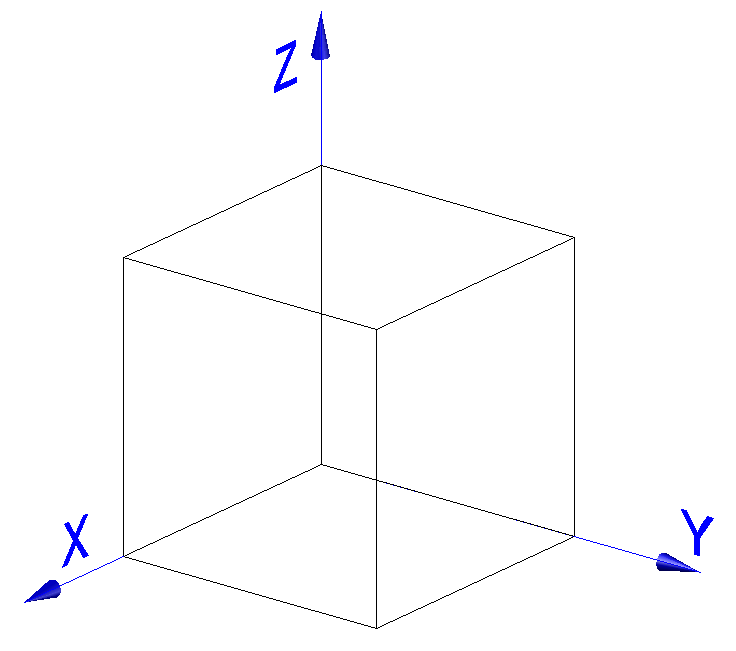
\includegraphics[scale=0.25]{pictures/cube1}
	\caption{Search Space.}
	\label{fig:cube1}
	\end{minipage}
	\hspace{0.5cm}
	\begin{minipage}[b]{0.5\linewidth}
	\centering
	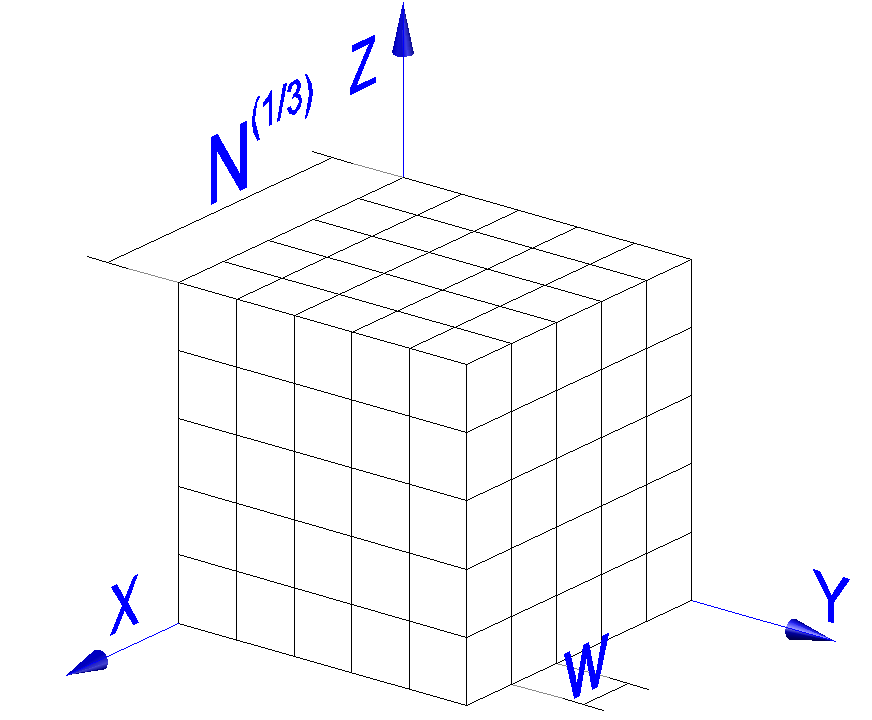
\includegraphics[scale=0.25]{pictures/cube2}
	\caption{Division of the search space in cells.}
	\label{fig:cube2}
	\end{minipage}
	\end{figure}  
	The Alg. \ref{alg:construct_search_space} gives more details about the construction of the space. It receives the cube size $N^{(1/3)}$, and the cell size \emph{W}.
	\begin{algorithm}
		\caption{Construct Search Space}
		\label{alg:construct_search_space}
		\begin{algorithmic}
		\STATE $discretized\_search\_space = \{\}$
		\STATE $max\_coord = N^{(1/3)}$
		\STATE $cell\_center = W / 2$
		\STATE $total\_number\_of\_cells = ceil(max\_coord / W)$
		\FOR{$x = 1 \to total\_number\_of\_cells$}
			\FOR{$y = 1 \to total\_number\_of\_cells$} 
				\FOR{$z = 1 \to total\_number\_of\_cells$}
					\STATE $discretized\_search\_space += (x * W + cell\_center,  y * W + cell\_center, z * W + cell\_center)$
				\ENDFOR
			\ENDFOR
		\ENDFOR
		\RETURN $discretized\_search\_space$
		\end{algorithmic}
	\end{algorithm}
	In the first instruction we begin by defining an empty search space. Then we define the maximum coordinate of our problem. It is important to say that our cube is only defined in the non-negative side of the xx, yy, zz axis (Fig. \ref{fig:cube1}). After this we calculate the center of each cell in terms of (x,y,z) components and add it to the new search space. 
	The return value is the discretized search space.
	
	The cells that are part of the discretized search space are then used as components $C$ of $G$ that the ants use to build solutions. The edges $E$ are arcs connecting all the components of the graph. In the following sections we will use the name \emph{cells} indistinctively.
	%\pagebreak
	\subsection{Initialize Pheromones}
	Before we start the optimization process, we need to initialize the pheromone matrix. This matrix contains the information about the quantity of pheromones of a certain path, and therefore it plays an important role in process of building solutions. For example, in the TSP the pheromone matrix contains information about how many times a certain path from city $i$ to city $j$ has appeared in a good solution.\\
	In cluster geometry optimization problems what is important is the position of atoms in space, and not the order in which they are placed. Therefore in DACCO, we are not interested in building paths, but place atoms in cells. Thus, instead of having information about how many times we have gone from cell $i$ to cell $j$, we have information about the desirability of having a certain component $i$ in a solution (i.e. placing an atom in a cell $i$).
	
	In the beginning of the algorithm, all the cells have the same desirability of being in a solution, and for that reason we initialize the pheromone matrix with the value of $0.5$, as in \cite{blum04}.
	\subsection{Construction of Solutions}
	The construction of solutions is achieved by the method Construct Solutions. An ant solution corresponds to a complete atomic cluster. The algorithm starts by defining a start position for the ant, thus we have to place the ant in a cell of our search space. Then the ant calculates which are the neighbors of it, and chooses, in a probabilistic way, a new cell to move. After it knows which cell is the next, it places the atom in the center of the current cell, adds it to solution, and moves to next one. This process is repeated until each ant has a cluster with all the atoms in place. The general algorithm that defines this construction process is detailed in Alg. \ref{alg:construct_solutions}.
	
	\begin{algorithm}
		\caption{Construct Solutions}
		\label{alg:construct_solutions}
		\begin{algorithmic}
		\STATE Given an ant \bf{do}:
		\STATE $placed\_elements = 1$
		\WHILE{$placed\_elements < N$}
			\STATE $neighbors = find\_feasible\_neighborhood(ant)$
			\STATE $next\_cell = find\_next\_cell(ant, neighbors, pheromone\_matrix)$
			\STATE $ant.solution[placed\_elements] = Atom(ant.current\_cell)$
			\STATE $ant.current\_cell = next\_cell$
			\STATE $placed\_elements = placed\_elements + 1$			
		\ENDWHILE
		\end{algorithmic}
	\end{algorithm}
	\pagebreak
	In the end of Alg. \ref{alg:construct_solutions} an ant will have built a complete atomic cluster.
	
	In the following we explain:\\ the $find\_feasible\_neighborhood()$ and $find\_next\_cell()$. 
	
		\subsubsection*{Find Feasible Neighborhood}
		This procedure determines the cells that are available in the neighbor of the current position of an ant. To find these neighbors, we used some different techniques:
		\begin{enumerate}
			\item Moore Neighborhood
			\item Convex Hull
			\item Full Moore Neighborhood
		\end{enumerate}
	
		\paragraph*{Moore Neighborhood}
			This neighborhood is defined, in $\mathbb{R}^3$, by the cube that is centered in a the current cell (x0, y0, z0). The Moore neighborhood of range r can be defined by the set M of all points (x, y, z) that verify the following condition:
			\begin{equation}
				M= \{(x,y):|x-x0| \leq r \wedge |y-y0| \leq r \wedge |z-z0| \leq r\}
			\end{equation}
			where $r \geq 0$. However, in our approach the values of r are only in the range r > 0, once we need to have at least one cell that is different from (x0, y0, z0). Fig. \ref{fig:moore_neighborhood} depicts the a Moore neighborhood with $r = 1$. We use a 2D representation for simplicity. 
			
			\botapic[0.50]{moore_neighborhood}{The grey cells represent the final M set, with $r = 1$}
			
			The final M set will then be used to determine which cell will be the next.
			
			\paragraph*{Convex Hull}
			With this technique we wanted to use more information about the problem, in the choice of the neighbors. Since the Morse potential takes in account the distance of all pair of atoms that composes the aggregate, we thought that we should use the information of the partially constructed solution to help choose the neighborhood. One of the first ideas that came into mind was the following: build a convex hull, with the atoms that are in the partial solution, and then determine all the cells that are at distance one from the segments defined by the points of the convex hull. The process is detailed in Alg. \ref{alg:convex_hull}.
			\begin{algorithm}
				\caption{Convex Hull}
				\label{alg:convex_hull}
				\begin{algorithmic}
				\STATE Given a partial solution of an ant \bf{do}:
				\STATE $ch = find\_convex\_hull(partial\_solution)$
				\FOR{$i = 1 \to length(ch)$}
					\FORALL{cells $CL$ of $discretized\_search\_space$}
						\IF{$(distance(CL, segment(ch[i-i], ch[i])) = 1$}
							\STATE $neighbors = neighbors \cup CL$
						\ENDIF
					\ENDFOR
				\ENDFOR
				\STATE $M = remove\_repeated\_cells(neighbors)$
				\RETURN $M$
				\end{algorithmic}
			\end{algorithm}
			
			The $remove\_repeated\_cells()$ procedure removes the repeated cells that are in the M set, since one cell can be in more the one atom neighborhood.
			The M set will then be used to determine which cell should be added to the solution.

			This technique uses the information of all the atoms that had already been placed, but it demands a lot of computational resources. Every time we place a new atom we have to calculate the Convex Hull of the current partial solution. This, together with the additional time on the calculus of the distance of all cells to the segments, we decided to consider other alternatives.
			
			\paragraph*{Full Moore Neighborhood}
			This technique was another attempt to use information about the partial constructed cluster. Here we iterate by all atoms that are in the partial solution, and we look for the neighbors of them. The neighborhood that we use is the Moore neighborhood with the same $r$ for all the atoms. The general idea is depicted in Fig. \ref{fig:all_neighbors}. We use a 2D representation for simplicity. The following algorithm gives more details about this technique:
		
			\begin{algorithm}
				\caption{Full Moore Neighborhood}
				\label{alg:all_atom_neighbors}
				\begin{algorithmic}
				\STATE Given a partial solution of an ant \bf{do}:
				\FOR{$i = 1 \to length(ch)$}
					\FORALL{atoms $AT$ of $partial\ solution$}
						\STATE $neighbors = neighbors \cup Moore\_Neighborhood(AT)$
					\ENDFOR
				\ENDFOR
				\STATE $M = remove\_repeated\_cells(neighbors)$
				\RETURN $M$
				\end{algorithmic}
			\end{algorithm}
		
		
		\botapic[0.50]{all_neighbors}{The grey cells represent the final M set, with $r = 1$}	
		
		\subsubsection*{Find Next Cell}	
		This procedure receives the feasible neighborhood and determines the next cell to be part of the solution. This means that, an ant, located in a cell $i$ should choose a new cell $j$ to add to the solution. This choice is based on the pheromone value of cell $j$, $\tau_{j}^{\alpha}$ and the heuristic information $\eta_{j}^\gamma$. It is important to say that we do not use the heuristic component of the choice function. The heuristic information is applied when we are building the feasible neighborhood. In the case of our problem we want to place atoms that are close to each other, and being so we can discard the cells that are too far away from the current one. 
		Taking this into account the choice function depends only of the pheromone value of cell $j$:
		\begin{equation}
			\label{eq:prob_rule}
			p_j = \frac{[\tau_j]^\alpha} {\sum_{l \in M} [\tau_l]^\alpha}
		\end{equation}
		
		Providing all values of the rule function are stored in an certain set $V$, the iterative cell selection is determined by a roulette wheel algorithm.: each value of the $V$ determines a slice on a circular roulette wheel. Next, the wheel is spun and the cell to which the marker points is chosen as the next cell for the ant. 
		In Alg. \ref{alg:find_next_cell} we detail the find next cell procedure, and in Alg. \ref{alg:roulette_wheel} we detail the roulette wheel selection method. 
		
			\begin{algorithm}
				\caption{Find Next Cell}
				\label{alg:find_next_cell}
				\begin{algorithmic}
				\STATE Given a set $M$ of candidate cells \bf{do}:
				\FORALL{cells in $M$}
						\STATE $V =$ Apply Eq. \ref{eq:prob_rule} the probability of each cell
				\ENDFOR
				\RETURN $roullete\_wheel(V)$
				\end{algorithmic}
			\end{algorithm}
			
			\begin{algorithm}
				\caption{Roulette wheel}
				\label{alg:roulette_wheel}
				\begin{algorithmic}
				\STATE Given a set $V$ of probabilities \bf{do}:
				\STATE $index = 0$
				\STATE $total = V[0]$
				\STATE pick a random value $r$ uniformly from $[0,1]$
				\WHILE{$total < r$}
					\STATE $index = index + 1$
					\STATE $total = total + V[index]$		
				\ENDWHILE
				\RETURN $index$
				\end{algorithmic}
			\end{algorithm}
			
			After finding the next cell, the ant will place the atom in its center, and then repeat all this process until it has a complete solution, that is, all the atoms have been placed.
			
			\subsection{Evaluate Solution in Continuous Space}
			
			The evaluation of the solutions built by the ants is made in this procedure. Since we have the atoms in the center of the cell, which are represented by $(x,y,z)$, where x, y, z $\in \mathbb{R}$, we do not have to make any additional computation to pass from the discretized space to the continuous space.
			
			The evaluation of the solutions proceeds in two steps. First, the Broyden-Fletcher-Goldfarb-Shannon (L-BFGS) quasi-Newton method \cite{liu89} move the solution to the nearest local optimum. Then equation \ref{eq:morse_potential} is used to determine the potential energy of the resulting cluster.

			L-BFGS is an efficient local optimization method that combines the modest storage and computational requirements of conjugate gradient methods with the super linear convergence exhibited by full memory quasi-Newton strategies. This local optimization algorithm is usually adopted by hybrid approaches for cluster geometry optimization problems \cite{grosso07, johnston03, xico09}.
						
			\subsection{Convert Solutions to Discrete Space}
			In this procedure we convert the solutions, which were returned by Evaluate Solutions in Continuous Space procedure, to the discrete space. This is very important, because the solutions returned after their evaluation are different from the ones that were given as parameters.
			To convert the cluster to the discretized space, we apply the following algorithm: given a certain atom, we move it to center of the nearest cell. This process is detailed in Alg. \ref{alg:convertion_discrete}.
			
			\begin{algorithm}
				\caption{Convert Solution to Discrete Space}
				\label{alg:convertion_discrete}
				\begin{algorithmic}
				\STATE Given a solution $CS$ in the continuous space \bf{do}:
				\FORALL{atoms $AT$ of $CS$}
						\FORALL{cels $CL$ of $discretized\ space$}
								\STATE $distances[AT][CL] = distance(AT, CL)$
						\ENDFOR
						\STATE $discrete\_solution = discrete\_solution \cup min\_dist\_cell(AT, distances)$
				\ENDFOR
				\RETURN $discrete\_solution$
				\end{algorithmic}
			\end{algorithm}
			
			The $min\_dist\_cell()$ procedure receives an array distance of atom to cells, and returns the cells that is closer to the atom in question.
			
			After this, we move all the cluster to the origin of the axis. This allows us to have the information concentrated in a place of the search space. 
			
			\subsection{Apply Discrete Local Search}
			This procedure is responsible for applying some perturbations in the solutions that were built by the ants, in an attempt to improve the search results.

			After the solutions have been converted to the discrete space, we look for the atom that has the worst contribution to the Morse potential, and we move it to a random cell.  After this, we evaluate the solution again, and if the result is a better solution, we keep it. This process is repeated for a given number of tries. The Alg. \ref{alg:discrete_local_search} gives a description of the process:
	
			\begin{algorithm}
				\caption{Apply Discrete Local Search}
				\label{alg:discrete_local_search}
				\begin{algorithmic}
				\STATE Given an ant solution AS\bf{do}:
				\STATE $i = 0$
				\STATE $best\_solution = AS$
				\STATE $current\_solution = AS$
				\WHILE{$i < local\_search\_iterations$}
					\STATE $worst\_atom\_cell = find\_atom\_worst\_contribution(current\_solution)$
					\STATE $new\_position = random\_cell()$
					\STATE $current\_solution[worst\_atom\_cell] = new\_position$
					\STATE $evaluate(current\_solution)$
					\IF{$is\_better(current\_solution, best\_solution)$}
						\STATE $best\_solution = current\_solution$
					\ELSE
						\STATE $current\_solution = best\_solution$
					\ENDIF
				\ENDWHILE
				\RETURN $best\_solution$
				\end{algorithmic}
			\end{algorithm}		
			
			The $local\_search\_iterations$ are the number of iterations that we make to try improve the solutions.	The $random\_cell()$ procedure returns a random cell that belongs to the search space, and that is not already occupied.mThe $is\_better()$ procedure checks if the first solution is better than the second one.
			\subsection{Update Pheromone Values}
			\botapic[0.50]{propagation}{Pheromone Propagation}
			This procedure is responsible for the update of the pheromones. We start by decreasing the current values of the pheromones, in a certain percentage, simulating the pheromone evaporation in the nature. After we follow the rule presented in \cite{blum04} to deposit pheromones, with some minor differences. In the cited approach, they used 3 ants to update the trails:
			\begin{enumerate}
				\item \emph{Iteration-best ant} - which corresponds to the best ant in the current iteration of the algorithm;
				\item \emph{Restart-best ant} - which corresponds to the best ant found since the restart of the algorithm
				\item \emph{Global-best ant} - which corresponds to the best solution found since the start of the algorithm
			\end{enumerate}
			
			However, in our approach we do not have a restart mechanism, thus we do not need to use the restart-best ant. 

			As was pointed out by \cite{blum04}, finding a schedule for the usage of the ants can be a difficult task, and it requires a lot of experimentation. However in the HyperCube Framework, we do not have this problem, because both iteration-best and global-best ants are allowed to deposit pheromones. The influence of each ant is measured by the weights that we assign to each one. The final rule to update pheromones is depicted as follows:
			\begin{equation}
				\tau = \tau + \omega
			\end{equation}
			
			where
			
			\begin{equation}
				\omega = w_{ib} * F_{ib} + w_{gb} * F_{gb}
			\end{equation}
			where $w_{ib}$ is the weight of the iteration-best ant, $F_{ib}$ is the quality of the iteration-best ant, $w_{gb}$ is the weight of the global-best ant, $F_{gb}$ is the quality of the global best ant, and $w_{ib} + w_{gb} = 1$.
			
			After the update is applied, pheromone values that exceed $\tau_{max}$ are set back to $\tau_{max}$. A similar process is applied to $\tau_{min}$.

			The final important aspect of the pheromone update rule is that the pheromones are not deposited in only in one cell. Instead, we only deposit a percentage $p$ in the main cell, and we propagate a percentage $(1-p)$ to the adjacent cells (Fig. \ref{fig:propagation}). This propagation is uniformly distributed among all the adjacent cells. This means that the value that is given to each one of the adjacent cells is $(1-p) / (number\ of\ adjacent\ cells)$. Such aspect is important to smooth the transitions between components in the search space.
			
			
		
		In appendix \ref{chap:implementation} we provide some technical decisions related with the implementation of this approach.
			
			
			
			
			